\documentclass[12pt, a4paper]{report}
\usepackage[top=1cm, left=1cm, right=1cm]{geometry}

\usepackage[utf8]{inputenc}
\usepackage[russian]{babel}

\usepackage{array}
\newcolumntype{M}[1]{>{\centering\arraybackslash}m{#1}}

\usepackage{hyperref}
\hypersetup{
	colorlinks,
	citecolor=black,
	filecolor=black,
	linkcolor=black,
	urlcolor=black
}

\usepackage{sectsty}
\allsectionsfont{\centering}

\usepackage{indentfirst}
\setlength\parindent{24pt}

\usepackage{makecell}

\usepackage{amsmath}

\def\H{\rule{0pt}{1.5ex}H}

\usepackage{graphicx}
\graphicspath{ {assets/initial/} {assets/results/} }
\usepackage[export]{adjustbox}
\usepackage{float}

\begin{document}
	\begin{titlepage}
		\begin{center}
			\large \textbf{Министерство науки и высшего образования Российской Федерации} \\
			\large \textbf{Федеральное государственное бюджетное образовательное учреждение высшего образования} \\
			\large \textbf{«Российский химико-технологический университет имени Д.И. Менделеева»} \\

			\vspace*{4cm}
			\LARGE \textbf{ОТЧЕТ ПО ЛАБОРАТОРНОЙ РАБОТЕ} \\
			\Large \textbf{Серментация частиц}

			\vspace*{4cm}
			\begin{flushright}
				\Large
				\begin{tabular}{>{\raggedleft\arraybackslash}p{9cm} p{10cm}}
					Выполнил студент группы КС-36: & Золотухин Андрей Александрович \\
					Ссылка на репозиторий: & https://github.com/ \\
					& CorgiPuppy/ \\
					& big-data-labs \\
					Принял: & Зубов Дмитрий Владимирович \\
					Дата сдачи: & 05.06.2025 \\
				\end{tabular}
			\end{flushright}

			\vspace*{5cm}
			\Large \textbf{Москва \\ 2025}
		\end{center}
	\end{titlepage}

	\tableofcontents
	\thispagestyle{empty}
	\newpage

	\pagenumbering{arabic}

	\section*{Описание задачи}
	\addcontentsline{toc}{section}{Описание задачи}
	\large
	Целью данной лабораторной работы являлась разработка и тестирование метода автоматического обнаружения и сегментации круглых частиц на микроскопических изображениях. Исходные данные представляли собой снимки (Рис. 1 и Рис. 2 в отчете) с масштабной меткой 50 nm, содержащие множество темных круглых частиц на светлом фоне. \par
	\textit{Основные задачи}:
	\begin{enumerate}
		\item Подготовка датасета путём вырезания фрагментов изображений различных размеров;
		\item Разметка частиц на изображениях с помощью инструмента \textit{Roboflow};
		\item Обучение модели компьютерного зрения для обнаружения частиц;
		\item Валидация модели на тестовых данных;
		\item Анализ качества работы модели на различных размерах изображений.
	\end{enumerate}

	\subsection*{Исходные данные}
	\addcontentsline{toc}{subsection}{Исходные данные}
	\large
	\begin{figure}[H]
		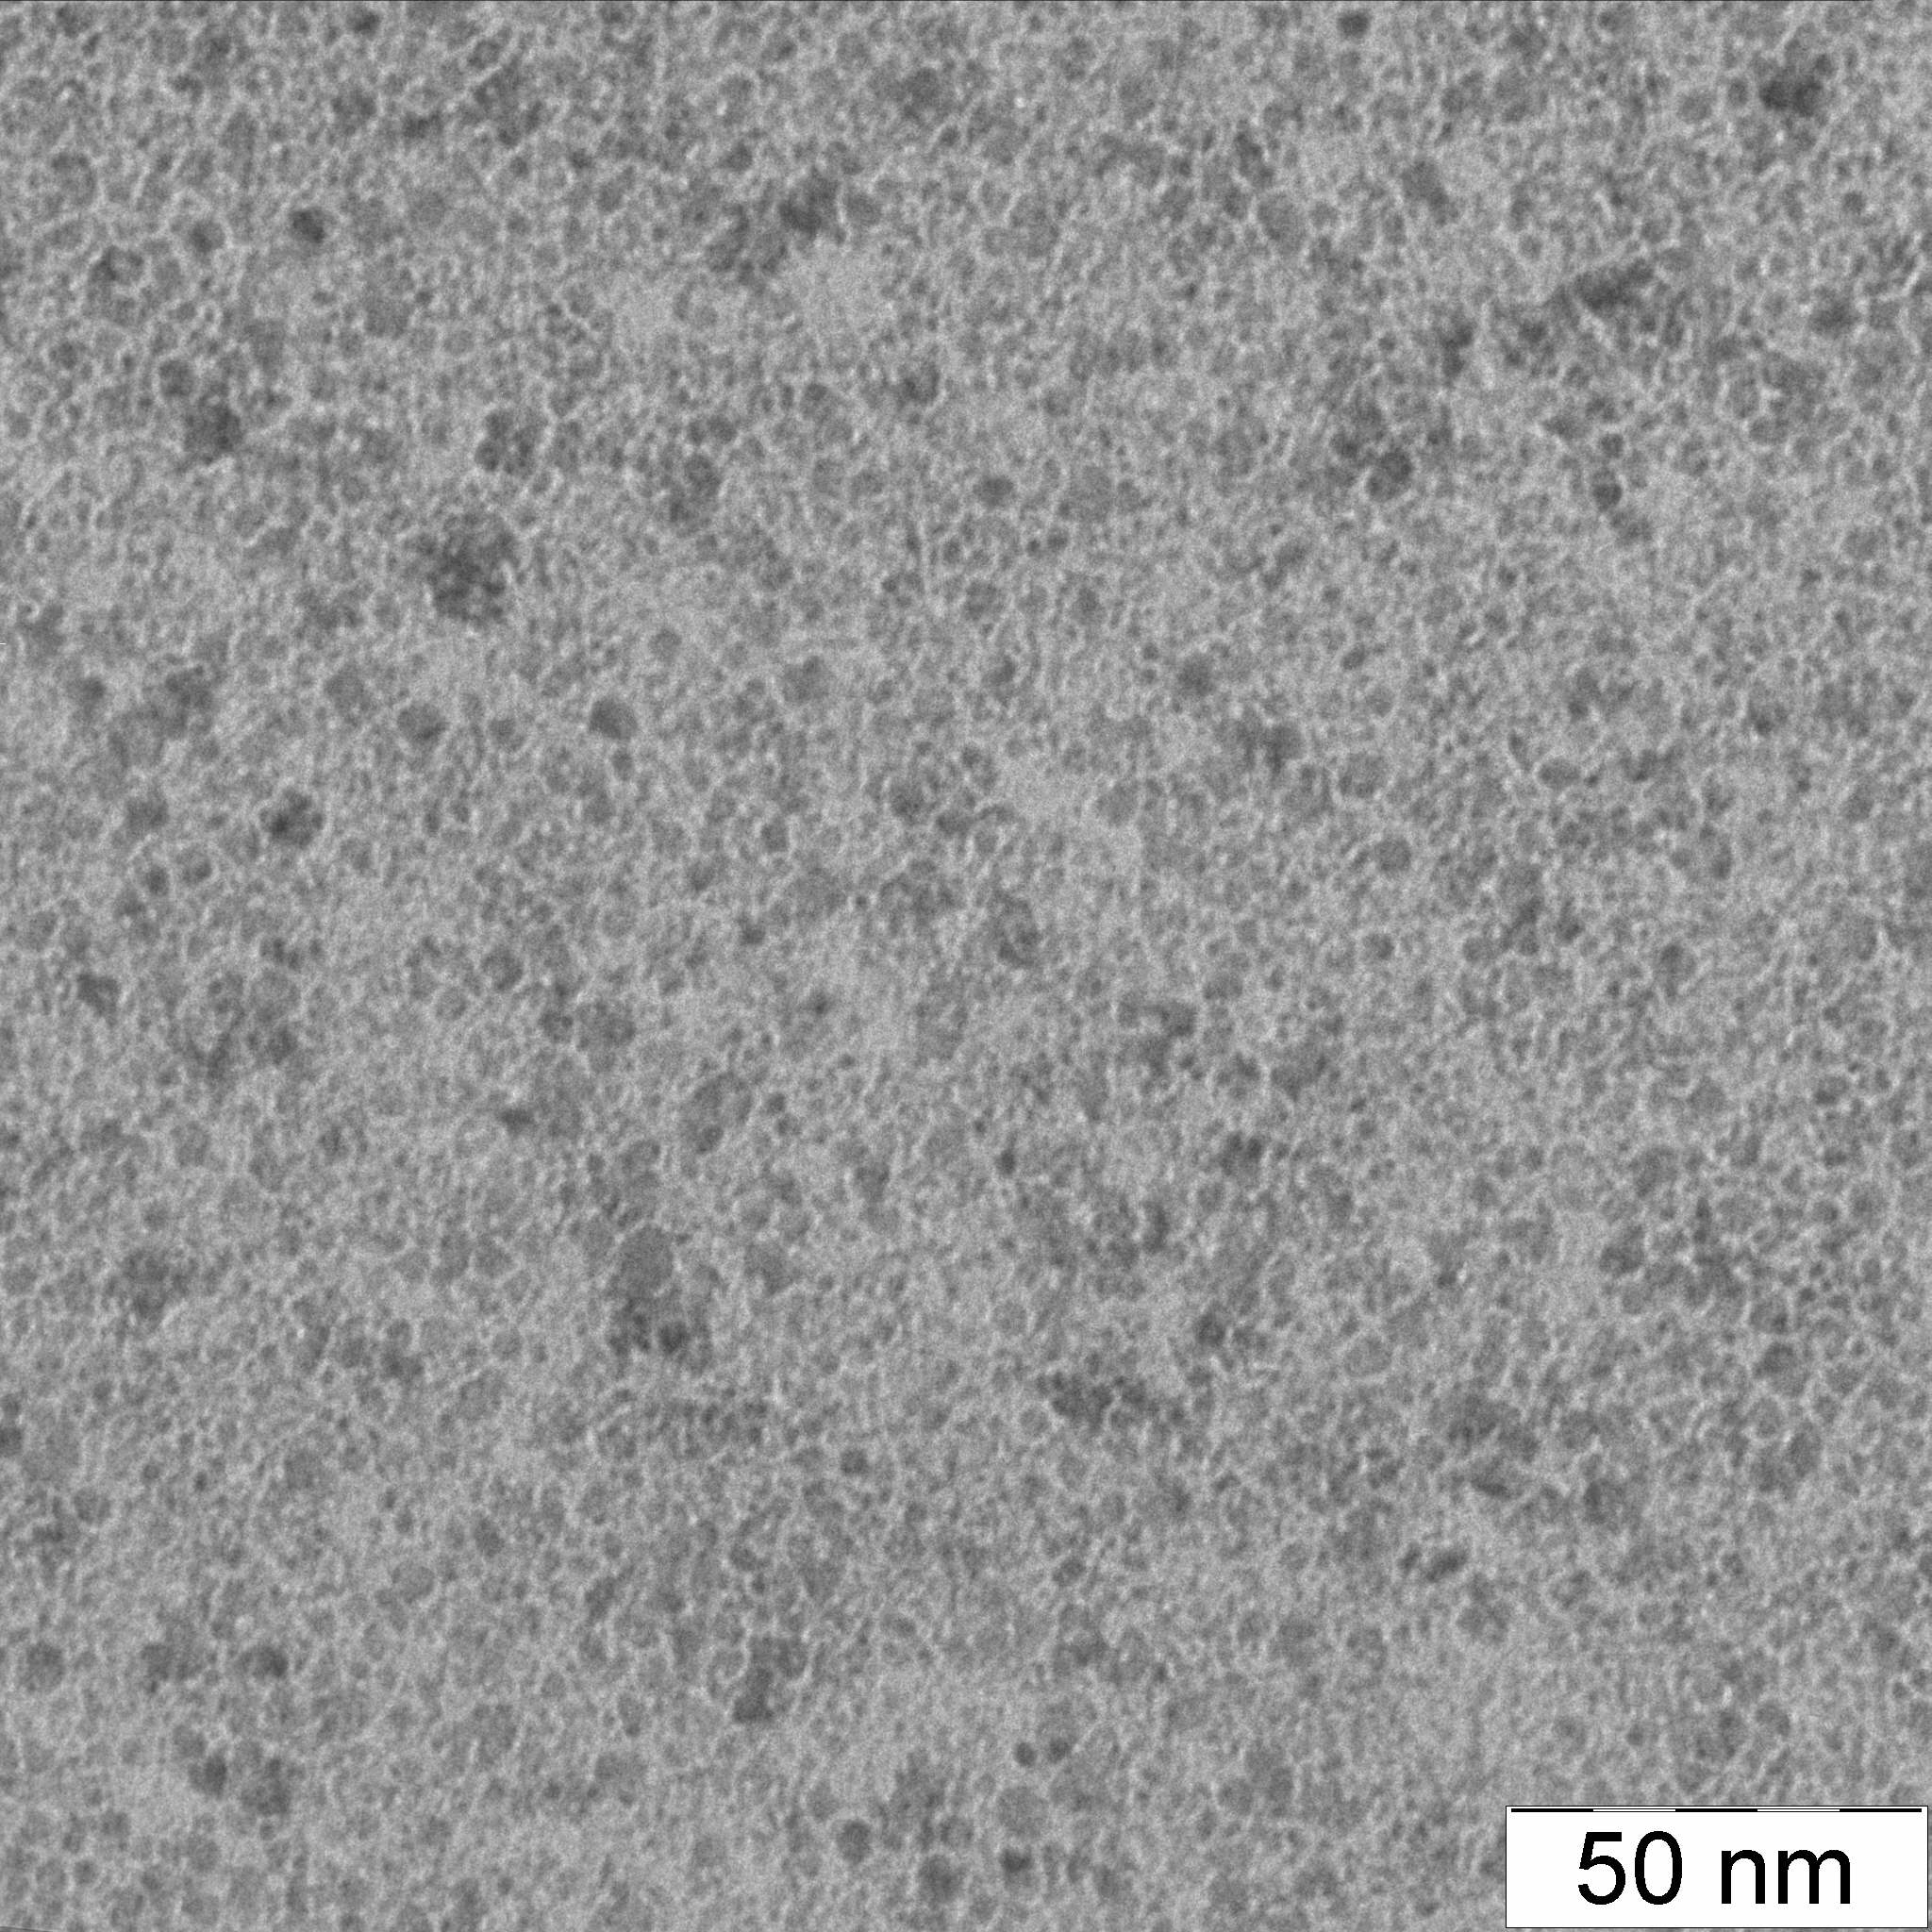
\includegraphics[width=300pt,center]{Image5.jpg}
		\caption{Снимок 5}
	\end{figure}
	\begin{figure}[H]
		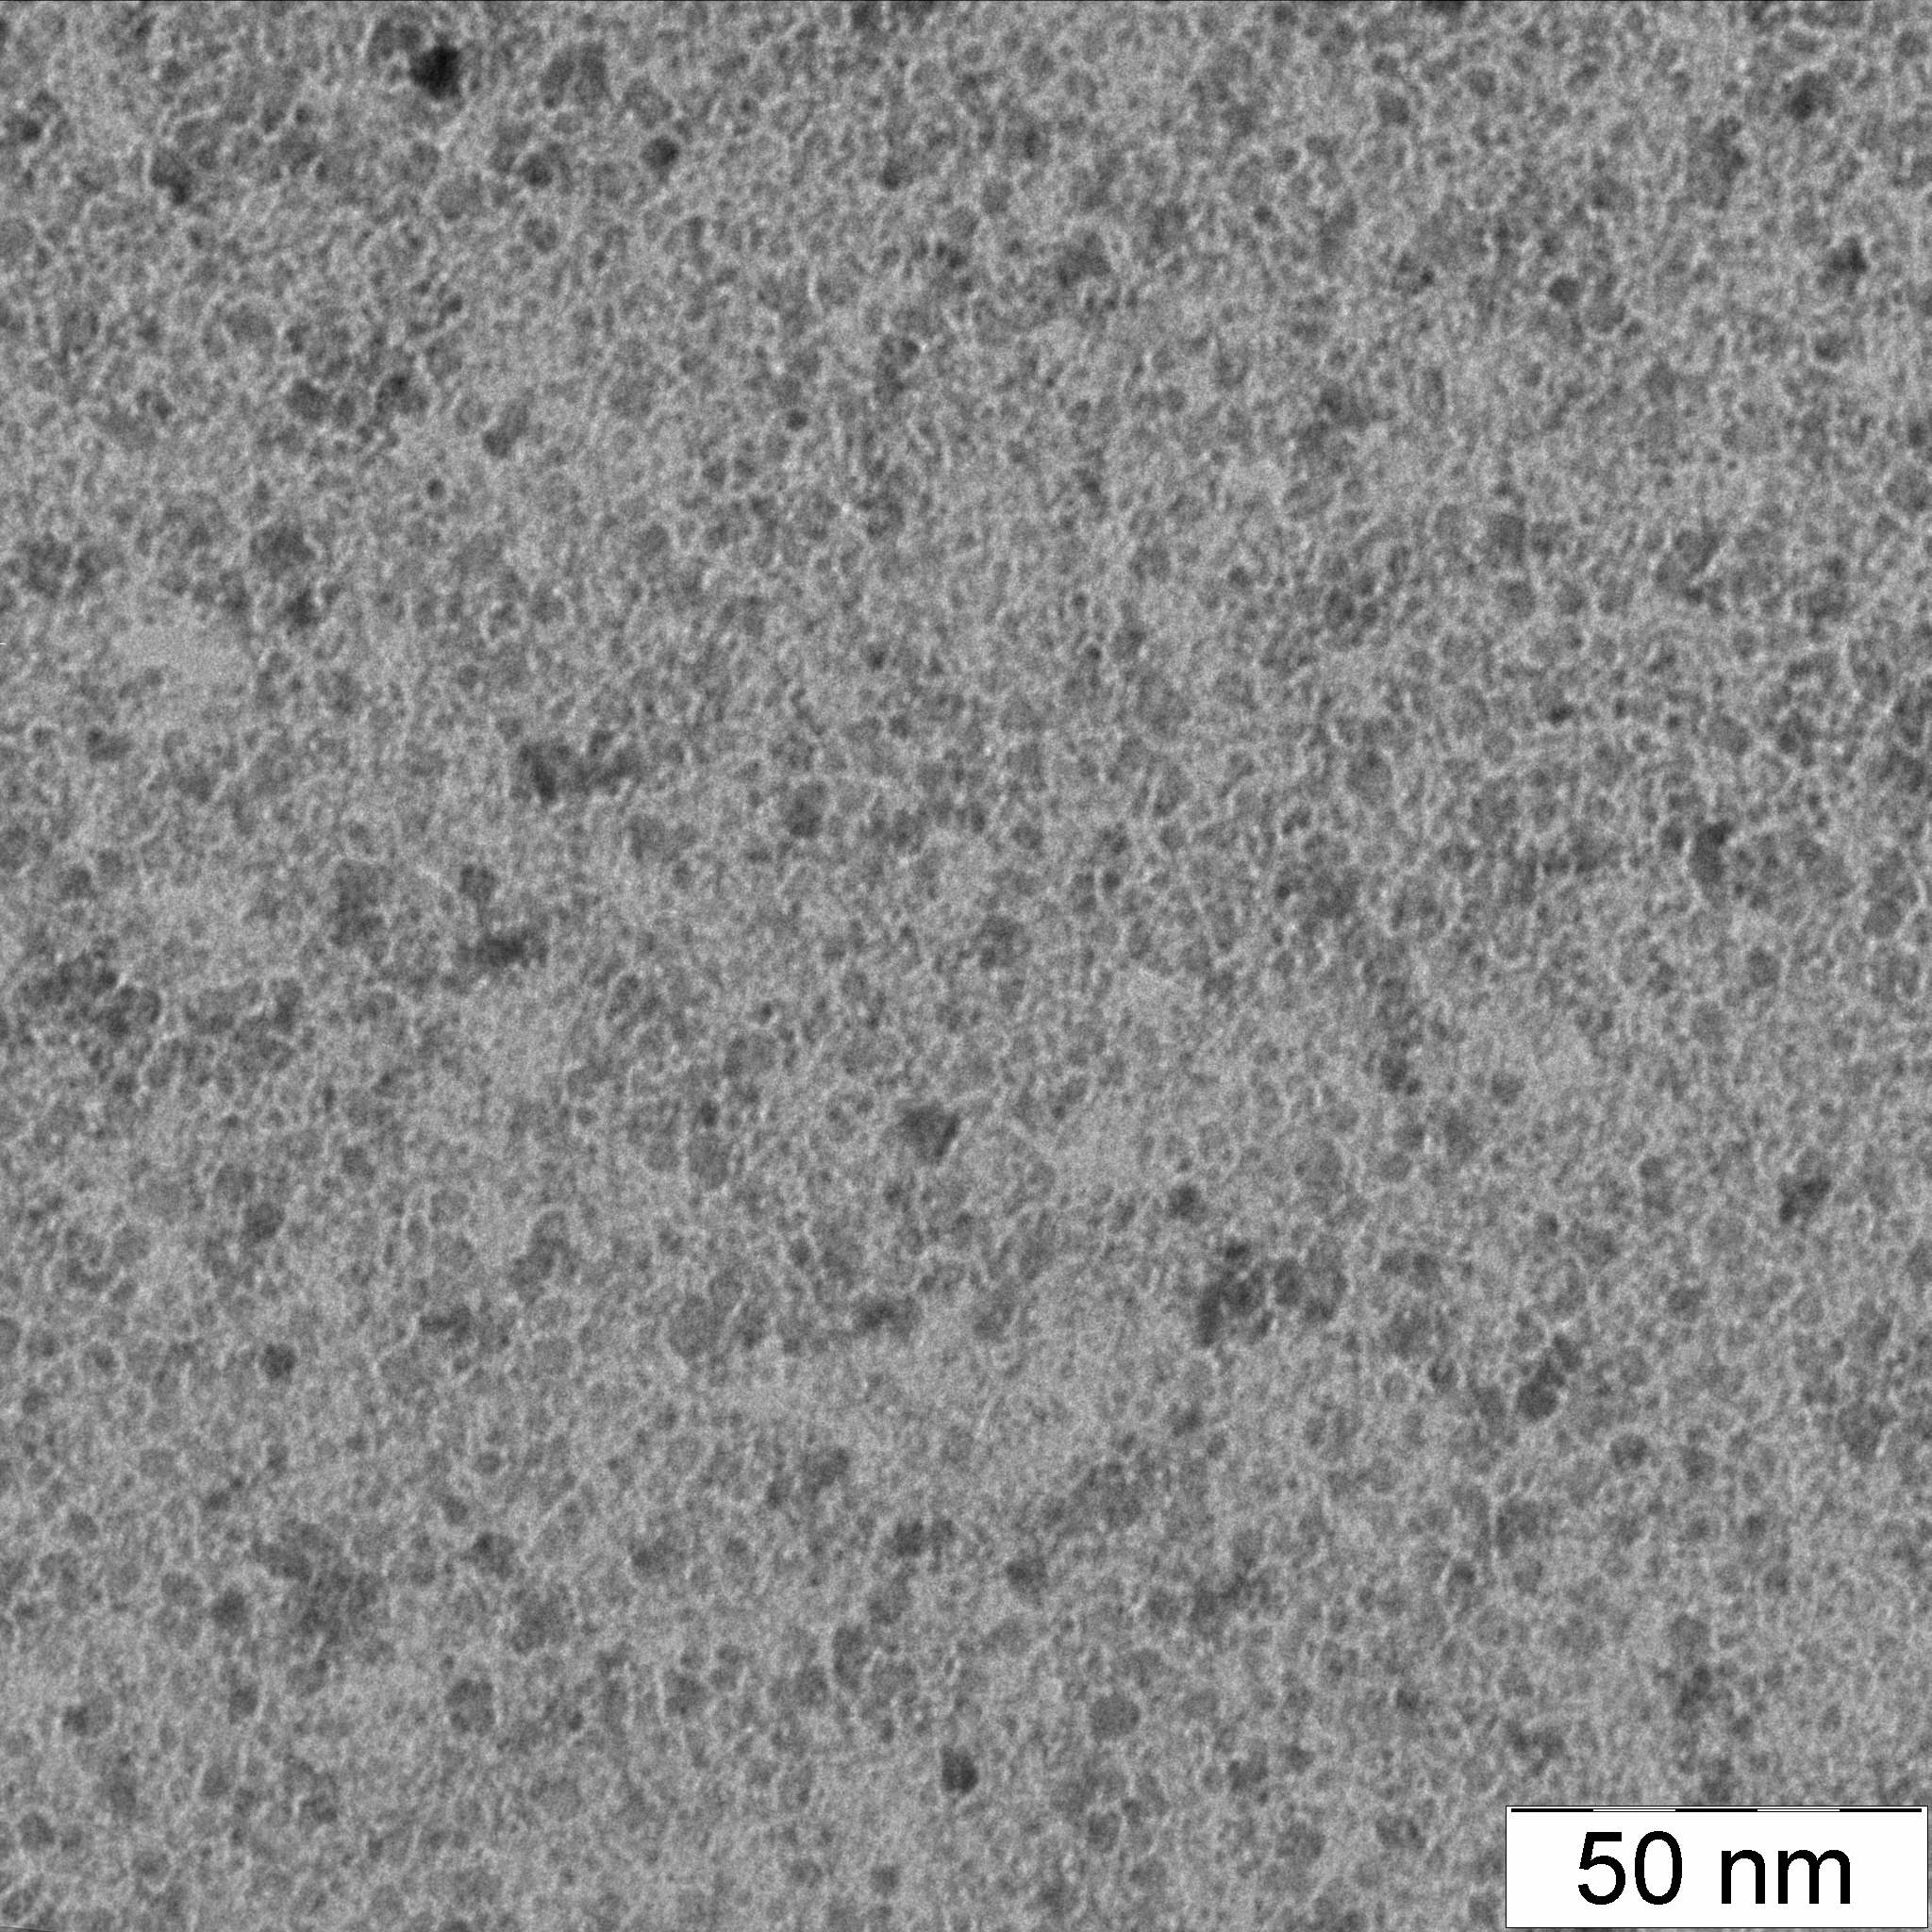
\includegraphics[width=300pt,center]{Image6.jpg}
		\caption{Снимок 6}
	\end{figure}

	\newpage

	\section*{Описание метода/модели}
	\addcontentsline{toc}{section}{Описание метода/модели}
	\large
	\begin{enumerate}
		\item Подготовка данных
		\begin{itemize}
			\item выполнение вручную разметки частиц на тренировочных изображениях с помощью Roboflow;
			\item создание bounding boxes вокруг каждой частицы;
			\item разделение датасета на обучающую и валидационную выборки.
		\end{itemize}
		\item Архитектура модели
		\begin{itemize}
			\item использована предобученнная YOLO-модель из Roboflow;
			\item модель основана на сверточных нейронных сетях;
			\item оптимизирована для обнаружения мелких объектов.
		\end{itemize}
		\item Процесс обучения
		\begin{itemize}
			\item обучение модели на размеченных данных;
			\item использование функции потерь, сочетающая классификацию и регрессию координат;
			\item применение аугментации данных для улучшения обобщающей способности.
		\end{itemize}
		\item Валидация
		\begin{itemize}
			\item тестирование проводится на изображениях различного размера;
			\item оценка качества по метрикам точности обнаружения и совпадения разметки.
		\end{itemize}
	\end{enumerate}

	\newpage

	\section*{Выполнение задачи}
	\addcontentsline{toc}{section}{Выполнение задачи}
	\large
	\begin{enumerate}
		\item Подготовка данных
		\begin{itemize}
			\item вырезаны фрагмента изображений указанных размеров;
			\item выполнена ручная разметка всех частиц на изображениях;
			\item данные загружены в Roboflow и разделены на Train/Valid наборы.
		\end{itemize}
		\item Обучение модели
		\begin{itemize}
			\item настроены параметры обучения (learning rate, batch size);
			\item запущен процесс обучения на облачной платформе Roboflow;
			\item мониторинг качества в процессе обучения.
		\end{itemize}
		\item Тестирование
		\begin{itemize}
			\item проверка модели на валидационных данных;
			\item анализ результатов на изображениях разных размеров;
			\item визуальная оценка качества обнаружения частиц.
		\end{itemize}
		\item Анализ результатов
		\begin{itemize}
			\item модель успешно обнаруживает большинство частиц;
			\item наблюдается хорошее соответствие между предсказанными и реальными границами;
			\item качество работы стабильно на изображениях разных размеров.
		\end{itemize}
	\end{enumerate}

	\newpage
	\vfill

	\subsection*{Подготовительные данные}
	\addcontentsline{toc}{subsection}{Подготовительные данные}
	\large

	\subsubsection*{Valid Dataset}
	\large
	\begin{figure}[H]
		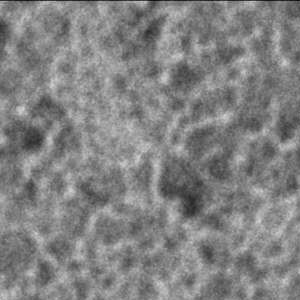
\includegraphics[width=250pt,center]{Image6_300_300.jpg}
		\caption{Вырезанное из снимка 6 изображние 300 на 300 пикселей}
	\end{figure}
	\begin{figure}[H]
		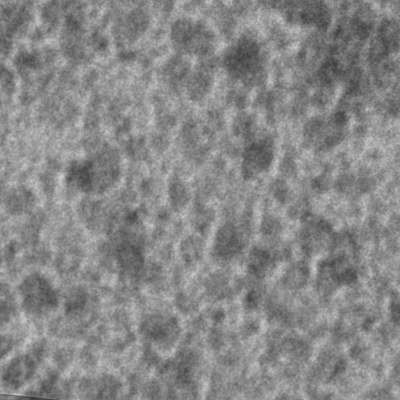
\includegraphics[width=250pt,center]{Image6_400_400.jpg}
		\caption{Вырезанное из снимка 6 изображние 400 на 400 пикселей}
	\end{figure}
	\begin{figure}[H]
		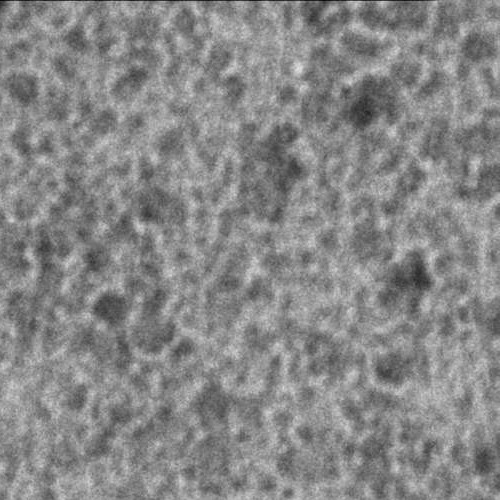
\includegraphics[width=250pt,center]{Image6_500_500.jpg}
		\caption{Вырезанное из снимка 6 изображние 500 на 500 пикселей}
	\end{figure}

	\newpage

	\subsubsection*{Test Dataset}
	\large
	\begin{figure}[H]
		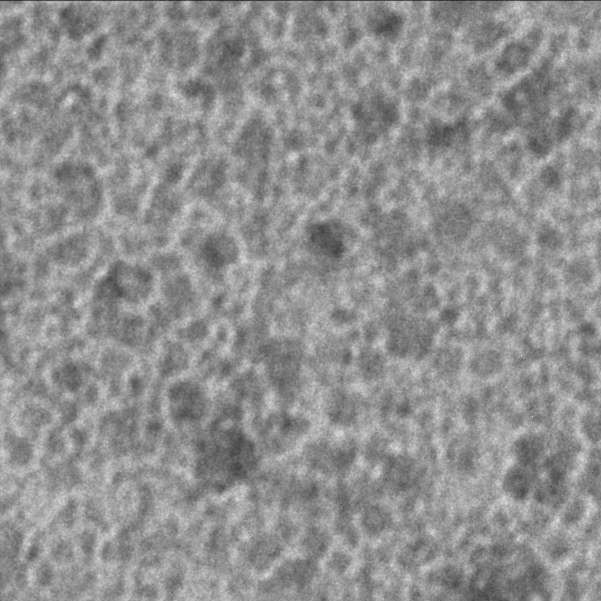
\includegraphics[width=250pt,center]{Image5_601_601.jpg}
		\caption{Вырезанное из снимка 5 изображние 601 на 601 пикселей}
	\end{figure}
	\begin{figure}[H]
		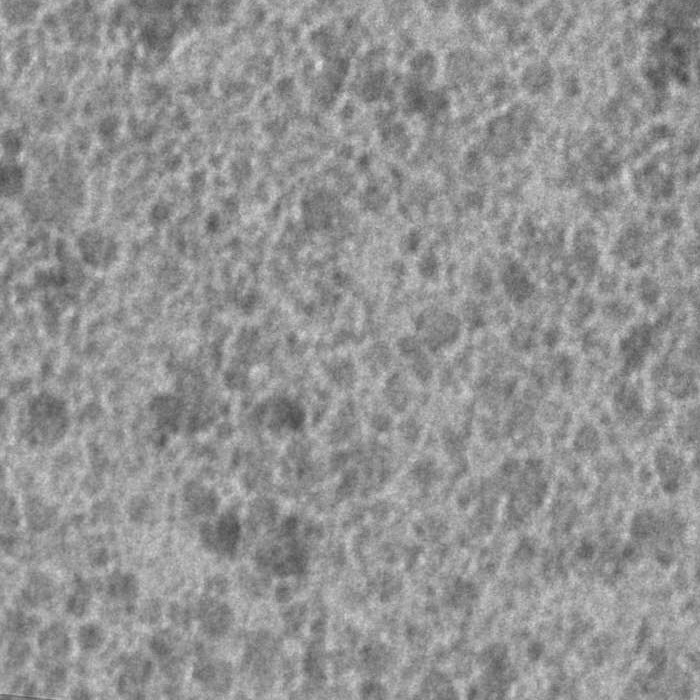
\includegraphics[width=250pt,center]{Image5_700_700.jpg}
		\caption{Вырезанное из снимка 5 изображние 700 на 700 пикселей}
	\end{figure}
	\begin{figure}[H]
		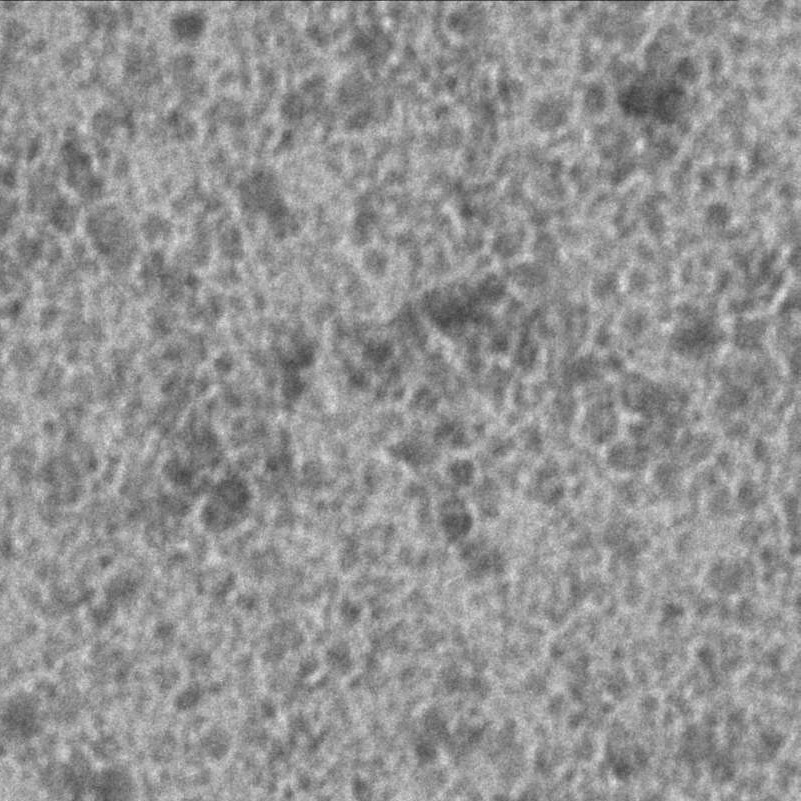
\includegraphics[width=250pt,center]{Image5_801_801.jpg}
		\caption{Вырезанное из снимка 5 изображние 801 на 801 пикселей}
	\end{figure}

	\newpage

	\subsubsection*{Train Dataset}
	\large
	\begin{figure}[H]
		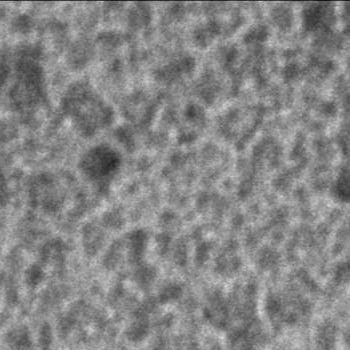
\includegraphics[width=250pt,center]{Image6_350_350.jpg}
		\caption{Вырезанное из снимка 6 изображние 350 на 350 пикселей}
	\end{figure}
	\begin{figure}[H]
		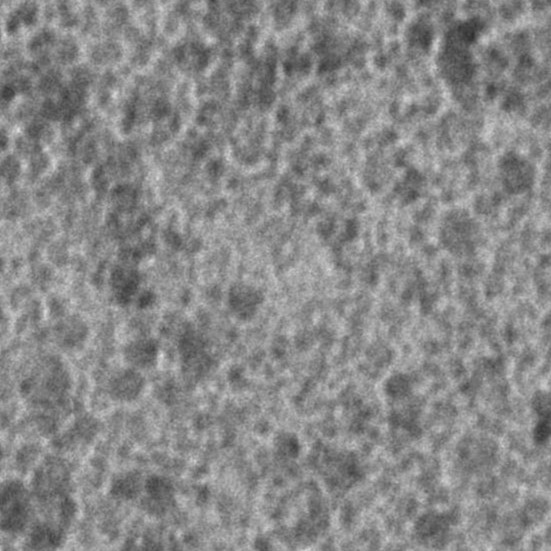
\includegraphics[width=250pt,center]{Image6_551_551.jpg}
		\caption{Вырезанное из снимка 6 изображние 551 на 551 пикселей}
	\end{figure}
	\begin{figure}[H]
		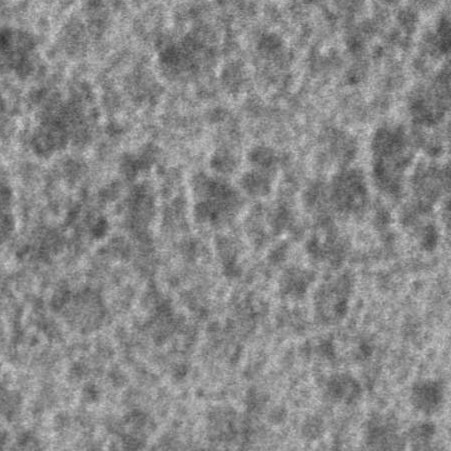
\includegraphics[width=250pt,center]{Image6_451_451.jpg}
		\caption{Вырезанное из снимка 6 изображние 451 на 451 пикселей}
	\end{figure}

	\subsection*{Результаты}
	\addcontentsline{toc}{subsection}{Результаты}
	\large
	\begin{figure}[H]
		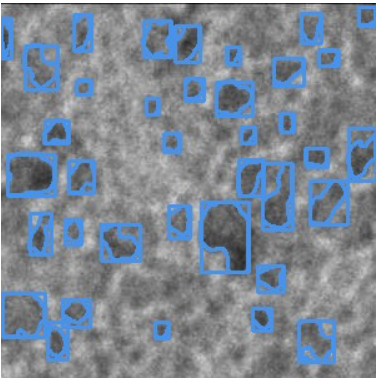
\includegraphics[width=250pt,center]{Image6_300_300_result.png}
		\caption{Результат вырезанного из снимка 6 изображeние 300 на 300 пикселей}
	\end{figure}
	\begin{figure}[H]
		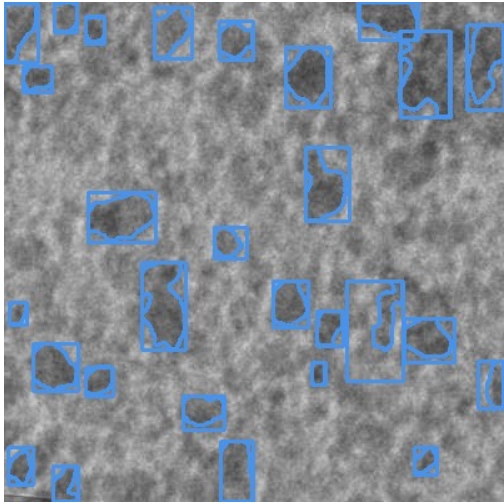
\includegraphics[width=250pt,center]{Image6_400_400_result.png}
		\caption{Результат вырезанного из снимка 6 изображeние 400 на 400 пикселей}
	\end{figure}
	\begin{figure}[H]
		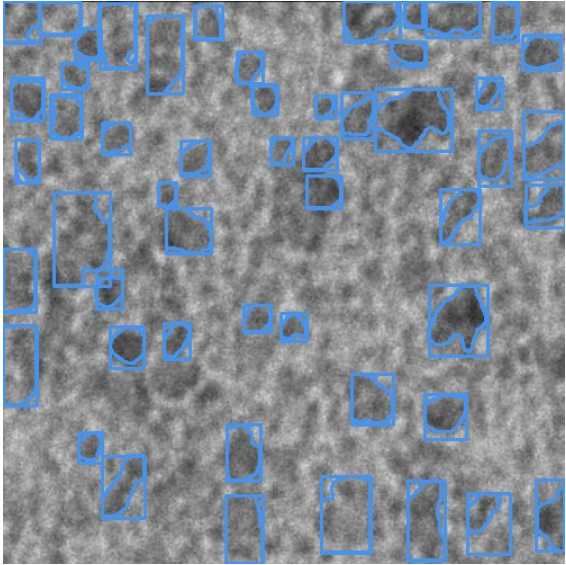
\includegraphics[width=250pt,center]{Image6_500_500_result.png}
		\caption{Результат вырезанного из снимка 6 изображние 500 на 500 пикселей}
	\end{figure}
	\begin{figure}[H]
		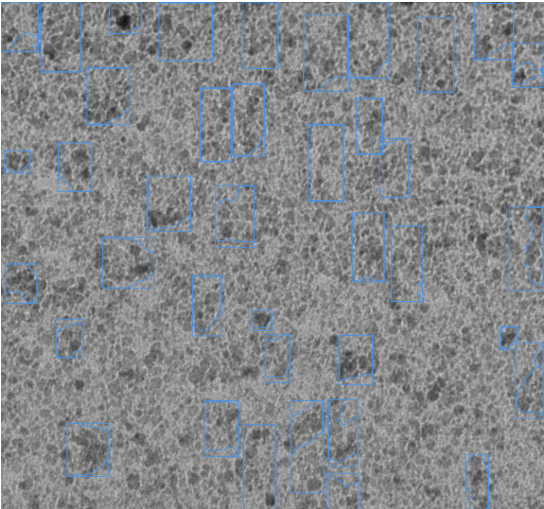
\includegraphics[width=250pt,center]{Image6_result.png}
		\caption{Результат снимка 6}
	\end{figure}

	\newpage

	\section*{Заключение}
	\addcontentsline{toc}{section}{Заключение}
	\large
	Как видно из представленных в отчете изображениях, модель успешно справляется с задачей обнаружения частиц нанометрового масштаба. Модель успешно идентифицирует отдельно расположенные частицы с четкими границами, что подтверждается результатами на валидационных изображениях различных размеров. \par
	Алгоритм испытывает трудности при обработке кластеров частиц, где происходит их взаимное перекрытие. В таких случаях часто происходит либо слияние нескольких частиц в один объект, либо пропуск части перекрытых частиц. \par
	Качество сегментации существенно зависит от равномерности освещения и контраста на исходных изображениях. На участках с неравномерной подсветкой возможны как ложные срабатывания, так и пропуск реальных частиц. \par
	Особые сложности возникают при обработке участков с высокой плотностью расположения частиц, где расстояние между ними сопоставимо с их размерами.
\end{document}
